 \begin{document}
% Set the page style to "fancy"...
\pagestyle{fancy}
%... then configure it.
\fancyhead{} % clear all header fields
\renewcommand{\headrulewidth}{0pt}
\renewcommand{\footrulewidth}{0pt}
\fancyhead[L]{\fontsize{16}{} \selectfont 42}
\fancyhead[C]{\textbf{К В А Н Т} · 2023/№4}
\fancyfoot{}
\setlength{\columnsep}{1cm}
\begin{multicols}{2}

\noindent равна $m_1 = \rho dS$. Предположим далее, что масса космолета $m=m_1=m_K=m_1(1+m_K/m_1)=\alpha m_1$, где $m_K$ - масса конструкций без учета паруса, $\alpha=1+m_K/m_1$ - конструкционный параметр парусного космолета. С учетом введенных параметров предельная скорость космолета, которую он приобретет за счет светового давления, будет равна
\[ \upsilon=\sqrt{\frac{2P_0Sr_0}{\alpha m_1}}=\sqrt{\frac{2P_0r_0}{\alpha\rho d}} \]
Из этой формулы следует, что предельная скорость солнечного парусника, приобретенная за счет давления света, не зависит от площади паруса. Зато она зависит от его толщины, плотности материала паруса и конструкционного параметра $\alpha$. В таблице приведены результаты расчетов предельной скорости $\upsilon$ для различных толщин, плотностей и параметров $\alpha$. Плотность $\rho=2,7 \cdot 10^3\, \text{кг/м}^3$ отвечает алюминию, плотность $\rho=1,6 \cdot 10^3\, \text{кг/м}^3$ - некоему гипотетическому материалу с высокой прочностью тонких пленок.
\bigskip\\
\renewcommand{\arraystretch}{1.3}
\setlength{\tabcolsep}{12pt}
\begin{tabular}{ |c|c|c|c|c| } 
\hline
№ & $d$,мкм & $\rho\text{,кг/м}^3$ & $\alpha$ & $\upsilon$,км/с \\ 
\hline
1 & 1,0 & 2700,0 & 1 & 31,2 \\ 
\hline
2 & 1,0 & 1600,0 & 1 & 40,6 \\ 
\hline
3 & 1,0 & 2700,0 & 2 & 17,5 \\ 
\hline
4 & 1,0 & 1600,0 & 2 & 28,7 \\ 
\hline
5 & 0,1 & 2700,0 & 1 & 99,0 \\ 
\hline
6 & 0,1 & 1600,0 & 1 & 128,5 \\ 
\hline
7 & 0,1 & 2700,0 & 1,5 & 80,8 \\ 
\hline
8 & 0,1 & 1600,0 & 1,5 & 105,0 \\ 
\hline
9 & 0,1 & 2700,0 & 2 & 55,2 \\ 
\hline
10 & 0,1 & 1600,0 & 2 & 92,0 \\ 
\hline
\end{tabular}\\
\bigskip

Как видно из приведенной таблицы, только в случае использования парусов из сверхтонких пленок толщиной 100 нм с плотностью порядка $1600,0\, \text{кг/м}^3$ солнечный парусник может достичь скорости, близкой к 105,0 км/с для конструкционного параметра, равного 1,5. Найдем для такого парусника площадь поверхности, необходимую для разгона космолета массой 1,0 т. С учетом $\alpha$ = 1,5 площадь паруса космолета будет равна

\[S=\frac{10^3}{1,5\cdot 1,6\cdot 10^3\cdot 10^{-7}}\, \text{м}^2\approx 4,2\cdot 10^6\, \text{м}^2=4,2\, \text{км}^2\]
Это достаточно большой парус. Создать для него прочную конструкцию будет непросто из-за больших размеров и очень малой толщины материала.
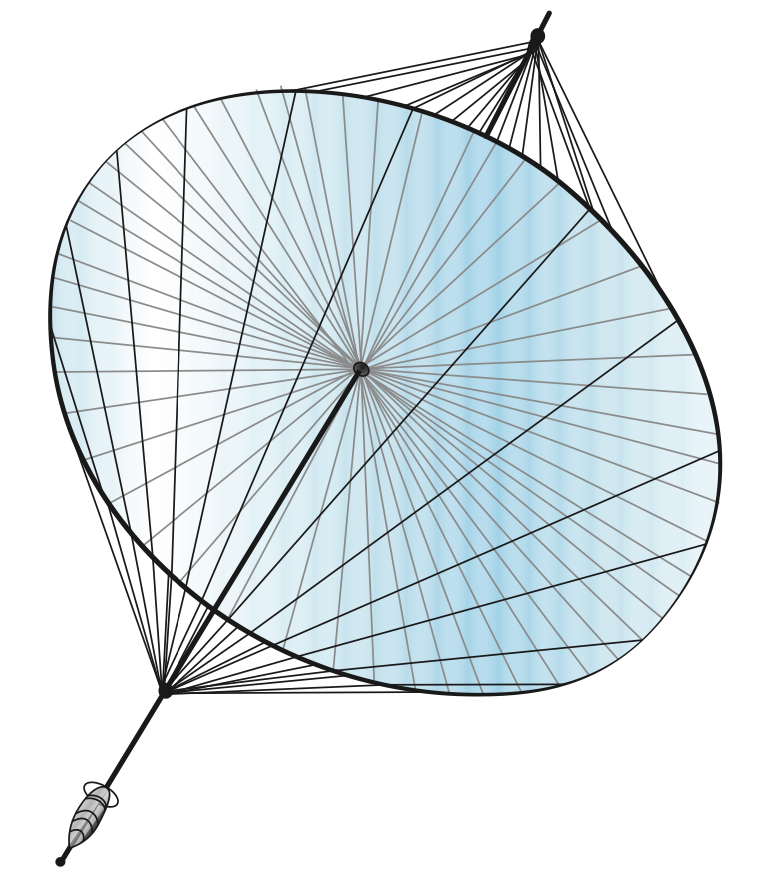
\includegraphics[scale=0.65]{picture}


На рисунке представлена возможная конструкция паруса сиспользованием тросов в качестве креплений солнечного паруса к корпусу космолета. Прочные тросы могут сделать конструкцию паруса жесткой и одновременно легкой. Подобная конструкция может быть использована и для создания космолетов на солнечной тяге для полетов с людьми. Правда, в этом случае придется собирать в космосе солнечные паруса площадью в сотни квадратных километров. С позиций современной космонавтики это исключительно сложная инженерно-техническая задача. Для ее решения понадобится разработать новые пленочные материалы для солнечных парусов с рекордными характеристиками по толщине, прочности и плотности. Все это отодвигает время появление солнечных парусников в отдаленное будущее. Подведем теперь небольшой итог изложенному материалу. Приведенные расчеты показывают, что использование давления сол-
\end{multicols}

\end{document}
